\chapter{Deep Neural Networks}

The history of artificial neural networks (ANN) dates back to 1943. In \cite{McCulloch1943} authors tried to mathematically describe the activity of biological neurons in the human brain. Using these principles they built a first artificial neuron and artificial neural network. In 1974 a PhD student, Paul Werbos, introduced in \cite{Werbos1974} the idea of backpropagation of errors by which ANN are able to learn other than linearly separable problems, and this idea was further expanded in \cite{Rumelhart1986}. Artificial neural networks that contain many hidden layers are also called deep neural networks (DNN) and the process of training this network is called deep learning \cite{LeCun2015}. Over the years deep learning and one of its variants - convolutional neural network that was proposed in \cite{LeCun2015-2} - were found to be very effective and precise in domains that were found unreachable by the classical AI and ML algorithms \cite{LeCun2015}. This was caused by their ability to capture abstract and complex patterns that simpler models found impossible to catch. Such examples include analysis of image data \cite{Farabet2013, Alzubaidi2021} and recent advancements in natural language processing (NLP) \cite{Deng2018}.

\section{Structure}
The fundamental part of every artificial neural network is the neuron. Neuron is basically a function which has one or more inputs and one output. Inside this neuron, a mathematical computation is being done in order to transform input into output. Input can also be referred to as input vector or vector of input features. Each input feature has its weight by which it is multiplied. Next, a bias is added to the multiplied and summed features and weights. This calculation is still linear so in order for it to be able to capture more complex patterns, we need to apply a non-linear activation function to its output. The mathematical representation of artificial neuron can be seen in the equations \ref{eq:linear} and \ref{eq:activation}.

\begin{align}
\label{eq:linear}
    z &= b + \sum_{i=1}^n (w_i x_i) \\
\label{eq:activation}
    a &= \varphi(z)
\end{align}

Where $z$ is the output produced by the linear unit, $b$ is the bias, $n$ is the number of input features, $x_i$ is the \textit{i}-th input feature, $w_i$ is the weight associated with the \textit{i}-th input feature, $a$ is the actual output, and $\varphi$ is the activation function.

Visual example of artificial neuron can be seen in figure \ref{fig:artificial-neuron}.

\begin{figure}[H]
\begin{centering}
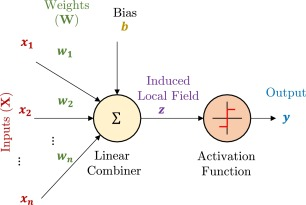
\includegraphics[width=8cm]{assets/images/neuron.jpg}
\par\end{centering}
\caption{Artificial neuron \cite{Santosh2022-1}}
\label{fig:artificial-neuron}
\end{figure}

\subsection{Activation Functions}
Activation functions are used to break linearity in neural networks - this enables them to capture more complex patterns, which are not linearly separable. Activation functions are used in combination with linear functions inside neurons. Different activation functions can be used, such as Sigmoid, Tanh, ReLU, ELU, GELU, and many more \cite{Dubey2022, Aby2025}.  The important part of an activation function is also its gradient, which is computed during backpropagation. 

\paragraph{Sigmoid}
Sigmoid is computed by the equation \ref{eq:sigmoid} and its derivative by the equation \ref{eq:sigmoid-derivative}. As we can see in figure \ref{fig:sigmoid} has a steep gradient around zero and it gradually flattens on both sides.

\begin{align}
\label{eq:sigmoid}
    \sigma(z) &= \frac{1}{1+e^{-z}} \\
\label{eq:sigmoid-derivative}
    \sigma^{'}(z) &= \sigma(z)(1-\sigma(z))
\end{align}

\begin{figure}[H]
\begin{centering}
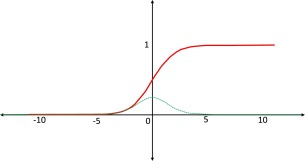
\includegraphics[width=8cm]{assets/images/sigmoid.jpg}
\par\end{centering}
\caption{Sigmoid activation function (red) and its derivative (green) \cite{Santosh2022-2}}
\label{fig:sigmoid}
\end{figure}

The output of the sigmoid is bound between zero and one, and its gradient can be used to push the output either closer to one or closer to zero \cite{Santosh2022-2}. It is often used for the output unit for the binary classification task, where the output is desired to be between zero and one \cite{Santosh2022-2, Goodfellow2016}.

\paragraph{Tanh} Next function is the \textit{tanh} activation function, given by the equation \ref{eq:tanh} and its respective derivative displayed on the equation \ref{eq:tanh-derivative}.

\begin{align}
\label{eq:tanh}
    \text{tanh}(z) &= \frac{e^z-e^{-z}}{e^z+e^{-z}} \\
\label{eq:tanh-derivative}
    \text{tanh}^{'}(z) &= 1-tanh^2(z)
\end{align}

Like the \textit{sigmoid} function, it compresses the input; however, unlike the \textit{sigmoid}, its output is constrained to the range of -1 to 1, as shown in figure \ref{fig:tanh}.

\begin{figure}[H]
\begin{centering}
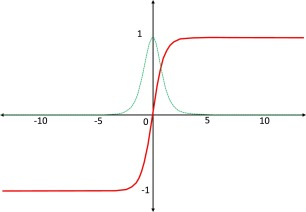
\includegraphics[width=8cm]{assets/images/tanh.jpg}
\par\end{centering}
\caption{Tanh activation function (red) and its derivative (green) \cite{Santosh2022-2}}
\label{fig:tanh}
\end{figure}

\paragraph{ReLU}
The problem with \textit{sigmmoid} and \textit{tanh} functions is the vanishing gradient and computational complexity. Vanishing gradient means that the gradient of a function is almost flat, hence close to zero, which leads to no or very little update in the network's learnable parameters (weights and biases) during the training \cite{Dubey2022, Aby2025}.

As a possible solution to these problems, a rectified linear unit, also known as ReLU, was introduced \cite{Nair2010}. ReLU is a simple function; its equation \ref{eq:relu} and derivative equation \ref{eq:relu-derivative} are straightforward.

\noindent
\begin{multicols}{2} % Two-column layout
    \begin{equation}
    \text{ReLU}(z) =
    \begin{cases} 
        z, & \text{if } z > 0, \\
        0, & \text{if } z \leq 0.
    \end{cases}
    \label{eq:relu}
    \end{equation}

    \begin{equation}
    \text{ReLU}'(z) =
    \begin{cases} 
        1, & \text{if } z > 0, \\
        0, & \text{if } z \leq 0.
    \end{cases}
    \label{eq:relu-derivative}
    \end{equation}
\end{multicols}

The ReLU function can be seen in figure \ref{fig:relu}. It basically returns its input if the input is positive otherwise, it returns zero. Since the derivative of \textit{x} is always one, the problem with vanishing gradient is solved. 

\begin{figure}[H]
\begin{centering}
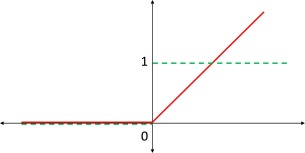
\includegraphics[width=8cm]{assets/images/relu.jpg}
\par\end{centering}
\caption{ReLU activation function (red) and its derivative (green) \cite{Santosh2022-2}}
\label{fig:relu}
\end{figure}

ReLU also introduces some potential drawbacks, i.e. the output for negative input is always zero. The problem called dying ReLU \cite{Dubey2022, Santosh2022-2, Aby2025} is when a negative input causes no updates in weights during training  and neurons in this state do not respond to error variations \cite{Santosh2022-2}. To fix this problem we can multiply the negative input value by a very small constant, which will allow the weights to be updated if it is needed. This modified ReLU is called Leaky ReLU \cite{Maas2013} and its formula and formula of its gradient are displayed in equations \ref{eq:leaky-relu} and \ref{eq:leaky-relu-derivative} respectively.

\noindent
\begin{multicols}{2} % Two-column layout
    \begin{equation}
    \text{LeakyReLU}(z) =
    \begin{cases} 
        z, & \text{if } z > 0, \\
        \alpha z, & \text{if } z \leq 0.
    \end{cases}
    \label{eq:leaky-relu}
    \end{equation}

    \begin{equation}
    \text{LeakyReLU}'(z) =
    \begin{cases} 
        1, & \text{if } z > 0, \\
        \alpha, & \text{if } z \leq 0.
    \end{cases}
    \label{eq:leaky-relu-derivative}
    \end{equation}
\end{multicols}

In addition to the Leaky ReLU, many other ReLU variants were introduced over the years, each bringing its own advantages, disadvantages, and challenges \cite{Dubey2022, Aby2025}.

Nowadays, the most commonly used activation function for hidden units is the ReLU activation function \cite{Dubey2022, Goodfellow2016, LeCun2015}.
% overview, traditional, new 

\subsection{Layers}

Similarly to biological neural networks, when artificial neurons are chained together, meaning the output from one neuron is passed to another neuron, they create an artificial neural network.

This network is organized in layers. Neurons in each layer are not connected together, but rather every neuron from layer \textit{L} is connected with every neuron from layer \textit{L+1}, except neurons in the first (input) layer. For better understanding, we will refer to the figure \ref{tab:artificial-nn} where we can see an example of a neural network.

\begin{figure}[H]
\begin{centering}
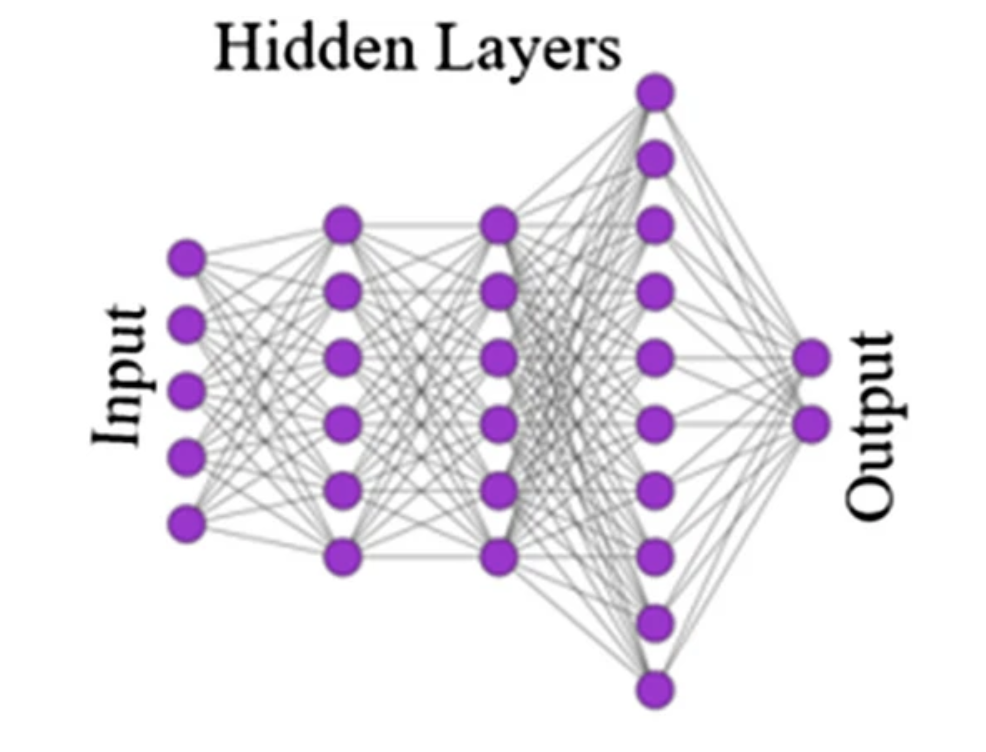
\includegraphics[width=8cm]{assets/images/neural_net.png}
\par\end{centering}
\caption{Example of deep artificial neural network \cite{TalaeiKhoei2023}}
\label{tab:artificial-nn}
\end{figure}

Neural network can be divided into three main parts:

\begin{itemize}
    \item Input layer
    \item Hidden layers
    \item Output layer
\end{itemize}

Input layer is the initial layer and the only layer that does not contain neurons which perform calculations but rather consists of \textit{N} input features $x_1, x_2, \dots, x_N$ also referred to as a vector $\vec{x}$ of input features:

\[
\vec{x} = \begin{bmatrix}
x_1 \\
x_2 \\
\vdots \\
x_N
\end{bmatrix}
\]

The subsequent layers between the input layer and output layer are called hidden layers. The name comes from the fact that their outputs are not directly observable, nor are they provided by the external environment - they are internal to the network's architecture. Neurons inside these layers perform calculations on the input and produce output, which is then fed forward to the next layer.

The final output layer produces an output of the network. Output and number of neurons depend on the task the network is being trained for. For regression tasks, one neuron is often suitable - it predicts a continuous variable \cite{Goodfellow2016}. During classification tasks, it can further depend on the nature of the classification. In binary classification, again a single neuron can suffice. It will display a probability of the input belonging to one of the classes - if the probability is high, it will assign that class to it, and if the probability is low, it will assign the other class to it \cite{Goodfellow2016}. In multi-class classification, the number of neurons is the same as the number of classes and each neuron predicts a probability of the input belonging to one specific class \cite{Goodfellow2016}.

\section{Loss Functions}
Loss function, sometimes also referred to as cost function, is a function that computes the difference between the result predicted by the model and the ground truth. This difference is called error. The error guides the model during training and is responsible for parameter updates. We are trying to find the local minimum of the cost function - a point where the error value is as low as possible, because this means that the model is making good predictions. Hence we are trying to find a global minimum of the cost function. Similarly to different activation functions, there is also a variety of cost functions.

\paragraph{Mean Squared Error}
Mean squared error (MSE) is computed as a sum of all differences between predicted output and real values (ground truth) raised to a power of two. The equation \ref{eq:mse} displays this computation, where $m$ is the number of input samples, $y$ is the ground truth, and $\hat{y}$ is the output predicted be the model. Despite being effective for regression problems, MSE is not that suitable for classification problems \cite{Santosh2022-2}.

\begin{align}
\label{eq:mse}
    E_\text{MSE} = \frac{1}{m}\sum_{i=1}^m(y_i-\hat{y}_i)^2
\end{align}

\paragraph{Cross-entropy Loss}
Much more efficient loss functions for classification problems are the entropy-based ones. For example, for binary classification, a logistic loss function, by which a binary cross-entropy error (BCE) is measured, is suitable \cite{Santosh2022-2}. It is given by the equation \ref{eq:logloss}, where $m$ is the number of input samples, $y$ is the ground truth, and $\hat{y}$ is the output predicted output.

\begin{align}
\label{eq:logloss}
    E_\text{BCE} = -\frac{1}{m}\sum_{i=1}^m(\hat{y}\log{y}+(1-\hat{y})(\log{(1-y)}))
\end{align}

This function can be modified to compute error for multiclass classification as well - this is also called categorical cross-entropy error (CCE). If we assume we have $C$ distinct classes we want to assign input into (and input can belong to exactly one class), then the equation \ref{eq:cce} computes the error. Here $m$ is the number of input samples, $C$ is a set of classes, $y_{i,c}$ is the ground truth for the \textit{i}-th sample and \textit{c}-th class, usually represented as a one-hot encoded vector where $y_{i,c}=1$ if the \textit{i}-th input belongs to the \textit{c}-th class, and $y_{i,c}=0$ and $\hat{y}_{i,c}$ is the predicted probability for the \textit{i}-th sample belonging to the \textit{c}-th class.

\begin{align}
\label{eq:cce}
    E_\text{CCE} = -\frac{1}{m}\sum_{i=1}^m\sum_{c=1}^C(y_{i,c}\log{\hat{y}_{i,c}})
\end{align}

\paragraph{Dice Loss}
The most popular choice for object segmentation task, and especially in the medical imaging domain, is the dice loss function \cite{Zhang2021}. It uses the Dice similarity coefficient (DSC) to compute the difference between predicted map $p$ and ground truth map $y$ for each class $j$ of $C$ classes. A slight problem exists with the DSC - it is not differentiable, therefore it cannot be used directly in training. To overcome this obstacle, neural networks use a probabilistic version of DSC to the discrete DSC in training \cite{Zhang2021}. Its computation is displayed in equation \ref{eq:dsc} where N depicts the number of pixels and $\epsilon$ is a small constant used to avoid division by zero. The computation of overall dice loss is displayed in equation \ref{eq:diceloss}, where $D_i$ is the DSC computed for the \textit{i}-th training sample.

\begin{align}
\label{eq:dsc}
\text{DSC}_i &= D_i = \frac{2 \sum_{n=1}^N \sum_{j=1}^C (y_{n,j} p_{n,j}) + \epsilon}{\sum_{n=1}^N\sum_{j=1}^C (y_{n,j} + p_{n,j}) + \epsilon} \\
\label{eq:diceloss}
E_\text{DiceLoss} &= \frac{1}{m}\sum_{i=1}^m (1-D_i)
\end{align}

\section{Training}
During the training phase, a neural network tries to minimize the cost function by adjusting its parameters - weights and biases. This process is often called learning, and we can say that the neural network learns to map input features onto the desired output. Prior to the training process we need to ensure that the data is in desired quality and quantity, otherwise the training will not be effective and the performance of the resulting model will be poor. Methods such as data preprocessing are typically used. 

Training itself consist of multiple steps:

\begin{enumerate}
    \item Parameter initialization
    \item Forward propagation
    \item Cost function computation
    \item Backpropagation and parameters updates
\end{enumerate}

\paragraph{Parameter initialization} During parameter initialization, we set the initial values of all learnable parameters of the network (parameters that can be updated during training). Different weight initialization strategies were developed, their overview can be seen in figure \ref{fig:init}.

\begin{figure}[H]
\begin{centering}
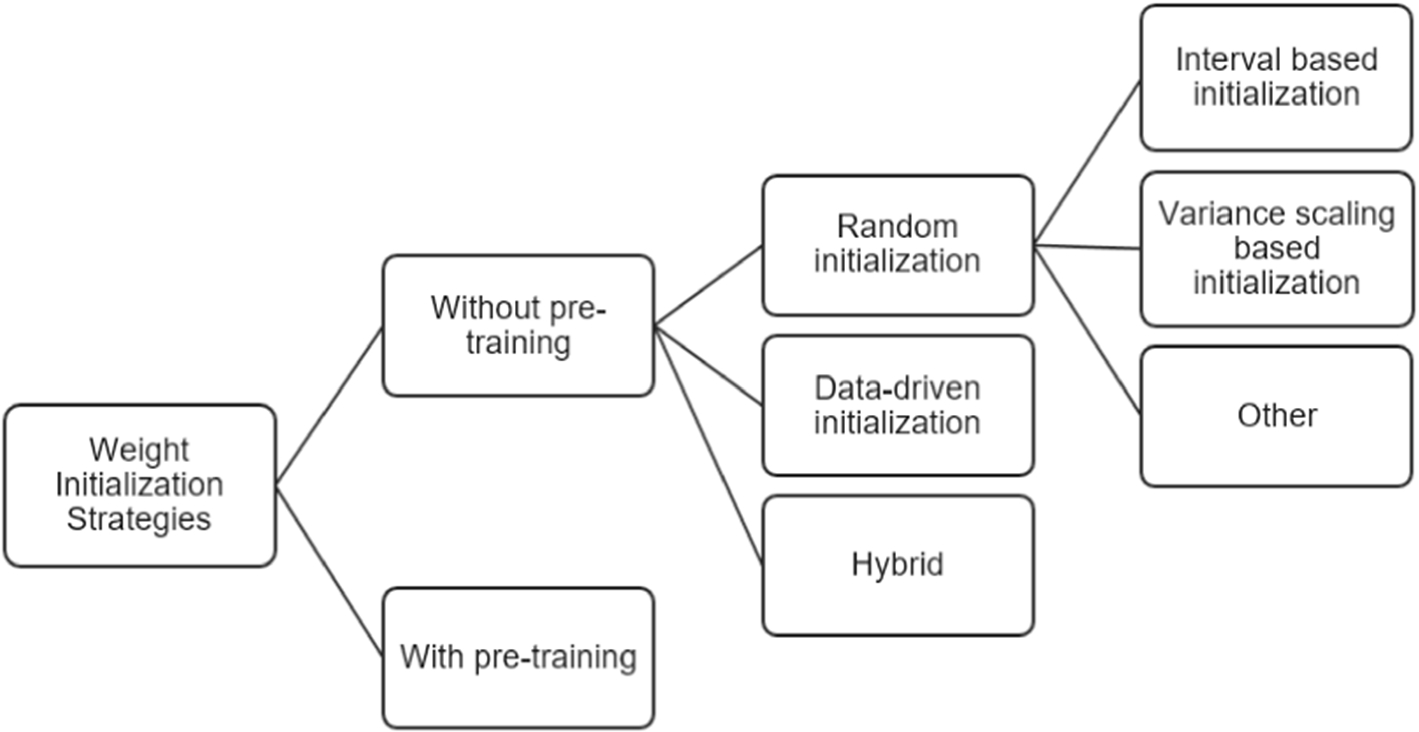
\includegraphics[width=8cm]{assets/images/init.png}
\par\end{centering}
\caption{Different weight initialization strategies \cite{Narkhede2021}}
\label{fig:init}
\end{figure}

Methods such as Xavier/Glorot or He initialization are also popular \cite{Abdullahi2023}.

\paragraph{Forward propagation}
During forward propagation the input sample data is fed forward through the layers of the network. For a hidden layer $L$ with $N$ neurons, and activation function $\varphi$:

\begin{itemize}
    \item The input is output from previous layer \textit{L-1} (the activations), denoted: $A_{L-1} \in \mathbb{R}^{m \times d}$, where $m$ is the number of input samples, and $d$ is the number of input features of each sample. Number $d$ is also equal to the number of neurons present in layer \textit{L-1}.
    \item Each neuron needs to have $d$ weights, one for each input feature. A weight matrix holding weights of all neurons in layer $L$ can then be denoted as: $W_L \in \mathbb{R}^{d \times N}$.
    \item Each neuron also holds a bias term, all biases in layer $L$ can be represented with vector $b_L \in \mathbb{R}^N$.
    \item Output matrix (the activations) returned by this layer can be denoted as: $A_L \in \mathbb{R}^{m \times N}$. This becomes input for the layer \textit{L+1}.
\end{itemize}

A computation performed by arbitrary hidden layer $L$ with $N$ neurons can that be calculated with equations \ref{eq:hidden-comp-z} - to compute $Z_L \in \mathbb{R}^{m \times N}$ pre-activation values, and \ref{eq:hidden-comp-a} - to compute output of layer $L$. Function $\varphi$ is applied element-wise on all elements of the input matrix.

\begin{align}
\label{eq:hidden-comp-z}
Z_L &= XW + b \\
\label{eq:hidden-comp-a}
A_L &= \varphi(Z)
\end{align}



The final output layer will then return the predicted output value for each sample. At the beginning of the training, the output values will be almost random, but as the training continues, the predicted values should converge towards the ground truth values - this is the desired behaviour.

\paragraph{Cost function computation}
After the sample (or samples) are fed forward through the network, we get either a matrix or vector of output values or a single output value. Next step is to compute the error of the network using one of the aforementioned cost functions, e.g. dice loss in case of image data. The error is than propagated backwards through the network and weights and biases are adjusted in a way that will minimize the cost function. This algorithm is called backpropagation.

\paragraph{Backpropagation}
In order for network to learn, it should implement some kind of algorithm, that will adjust its learnable parameters (weights and biases) in a way, that the overall error will be lower next time the input samples are fed forward through the network. Backpropagation computes the gradients for each layer starting with the output layer, and by utilizing the chain rule of calculus, it propagates the error back through the network to the first hidden layer.

After the gradients are computed, the parameters are updated accordingly by optimization algorithms such as stochastic gradient descent \cite{Santosh2022-2}. Formulas for updating weights and biases are shown in equation \ref{eq:w-update} and \ref{eq:b-update}, where $\alpha$ is a learning rate (which controls the speed of learning - if changes to the parameters are too great, the minimum can be missed, if changes are too small, the minimum will not be reached in a reasonable time) and $E$ is the cost function.

\begin{align}
\label{eq:w-update}
w &= w - \alpha \frac{\partial E}{\partial w} \\
\label{eq:b-update}
b &=  b - \alpha \frac{\partial E}{\partial b}
\end{align}

There is a strict rule for backpropagation to work - all functions used in the network must be differentiable at all points \cite{Rumelhart1986, Santosh2022-2}.

\subsection{Optimization and regularization}

\paragraph{Optimization}
There are many optimization techniques which are capable of further enhancing the model training and performance. Examples include:

\begin{itemize}
    \item using small batches of input samples and after each batch passes perform parameter updates,
    \item utilizing momentum \cite{Polyak1964} to have more control over the learning speed based on the previous gradients \cite{Santosh2022-2},
    \item using adaptive learning rates, where the learning rate $\alpha$ is usually great at the beginning and as the training progresses it is gradually reduced \cite{Santosh2022-2}. Updates to $\alpha$ can be done after some number of iterations by some preset factor or automatically by utilizing methods such as Adam (adaptive moments) \cite{Kingma2014} or RMSProp \cite{Zou2019}.
\end{itemize}

\paragraph{Regularization}
Another set of techniques that can improve model performance is regularization. Usually, a model's performance and prediction capabilities improve during training. Available data are often split into three subsets for training, validation, and testing. The model is, obviously, trained using the training subset. The validation subset is used to check model performance during training, and the test subset is used for the final evaluation of the model. It is important that both validation and test subsets contain samples the model has not yet seen during training - otherwise, the results would be biased. A good model should be robust and generalize well, not only learn patterns that are specific for training data. Sometimes, especially in more complex models, we can observe an effect when, at the beginning of the training, both training and validation performance (such as error value) improve, but later the validation performance plateaus or worsens - this effect is called overfitting \cite{Schaffer1993} and is displayed in figure \ref{fig:overfitting}. 

\begin{figure}[H]
\begin{centering}
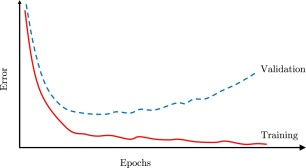
\includegraphics[width=8cm]{assets/images/overfitting.jpg}
\par\end{centering}
\caption{Error curve during training - overfitting happens \cite{Santosh2022-2}}
\label{fig:overfitting}
\end{figure}

This effect is not desired because it means that the model cannot generalize well on previously unseen samples - it is learning "by heart" from the training data. To overcome this problem, we can implement several regularization mechanisms, that will improve the model's robustness and ability to generalize. Examples include dropout \cite{Srivastava2014}, transfer learning \cite{Pan2009}, early stopping \cite{Sarle1996}, parameter norm penalties such as L1 regularization (lasso regression) and L2 regularization (ridge regression) \cite{Krogh1991}, and more \cite{Santosh2022-2}.



\section{Evaluation Metrics}
When evaluating a model's performance, various different metrics exist that can be used. The evaluation metrics also depend on the task the model was trained for. During classification tasks, depending on the predicted and real values for each sample, we can differentiate four groups of results:

\begin{itemize}
    \item True Positives (TP) - a model assigns a sample to class $c$, when a sample belongs to class $c$,
    \item True Negatives (TN) - a model does not assign a sample to class $c$, when a sample does not belong to class $c$
    \item False Positives (TP) - a model does assign a sample to class $c$, when a sample does not belong to class $c$
    \item False Negatives (TN) - a model does not assign a sample to class $c$, when a sample does belong to class $c$
\end{itemize}

We will briefly describe some of the evaluation metrics in the following paragraphs. 

\paragraph{Accuracy, Precision, Recall, and F1 Score} Calculation of these basic metrics is displayed in equations \ref{eq:accuracy}, \ref{eq:precision}, \ref{eq:recall}, and \ref{eq:f1}. They describe the relationships between the number of samples belonging to either the true positive (TP), true negative (TN), false positive (FP), or false negative (FN) groups.

\begin{align}
\label{eq:accuracy}
\text{Accuracy} &= \frac{TP + TN}{TP + TN + FP + FN} \\
\label{eq:precision}
\text{Precision} &= \frac{TP}{TP + FP} \\
\label{eq:recall}
\text{Recall} &= \frac{TP}{TP + FN} \\
\label{eq:f1}
\text{F1\ Score} &= 2 \times \frac{\text{Precision} \times \text{Recall}}{\text{Precision} + \text{Recall}}
\end{align}

\paragraph{Area Under the ROC Curve}
Receiver Operating Characteristics (ROC) Curve and area under it can be used as another evaluation metric for classification and is superior when compared to overall accuracy \cite{Bradley1997}. The ROC Curve is drawn in the ROC Space as a relationship between the True Positive Rate (TPR, Recall or Sensitivity) and False Positive Rate (FPR) at the different threshold levels \cite{Bradley1997, Nahm2022, Fawcett2006}; the calculation of TPR and FPR is shown in the equations \ref{eq:tpr} and \ref{eq:fpr}.

\begin{align}
\label{eq:tpr}
\text{FPR} &=\text{Specificity} = \text{Recall} = \frac{TP}{TP + FN} \\
\label{eq:fpr}
\text{FPR} &= 1-\text{Specificity} = \frac{FP}{FP + TN}
\end{align}

The ROC Space and example of ROC Curve is displayed in figure \ref{fig:roc}. Area under this curve (AUC - Area Under the ROC Curve) is then computed and interpreted:

\begin{itemize}
    \item if $\text{AUC} = 1$, this is the perfect model
    \item if $\text{AUC} = 0.5$, model capability is equal to random guess
    \item if $\text{AUC} < 0$, performance of the model is worse than the random guess
\end{itemize}

\begin{figure}[H]
\begin{centering}
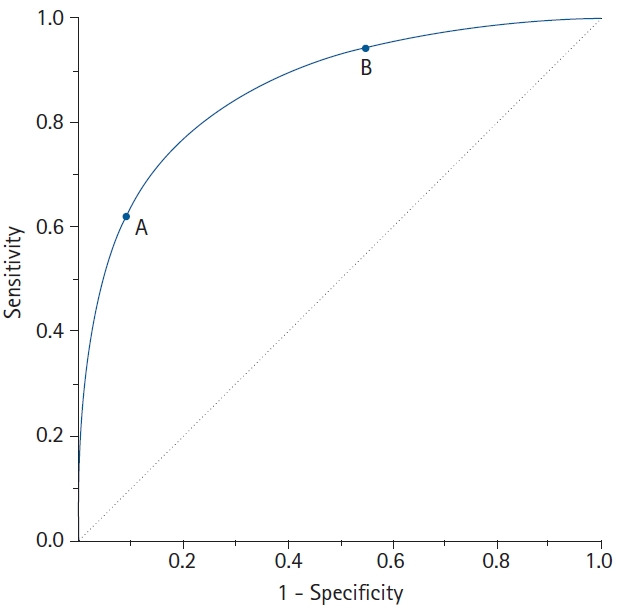
\includegraphics[width=8cm]{assets/images/roc-space.jpg}
\par\end{centering}
\caption{ROC Space with ROC Curve \cite{Nahm2022}}
\label{fig:roc}
\end{figure}

\paragraph{Intersection over Union} Intersection over Union (IoU), also known as the Jaccard Index, is a widely used evaluation metric in image segmentation and object detection \cite{Rezatofighi2019}. It is computed as the area of overlap between the predicted and ground truth regions divided by the area of their union. The closer the resulting value is to 1 the better the model predictions are \cite{Rezatofighi2019}. Its computation is shown in equation \ref{eq:iou}, where $y$ is the true area and $\hat{y}$ is the area predicted by the model.

\begin{align}
\label{eq:iou}
\text{IoU} &= \frac{y \cap \hat{y}}{y \cup \hat{y}}
\end{align}

\paragraph{Dice Coefficient} Similarly to the IoU, the Dice Coefficient is used for image segmentation and detection tasks \cite{Hu2023}, and the closer the resulting value is to 1 the better the model predictions are. Its computation is given by the equation \ref{eq:dice}, where $y$ is the true area and $\hat{y}$ is the area predicted by the model.

\begin{align}
\label{eq:dice}
\text{DiceCoefficient} &= \frac{2|y \cap \hat{y}|}{|y| + |\hat{y}|}
\end{align}